\chapter{Conceitos básicos}\label{cap_conceitos}

O foco deste capítulo é introduzir alguns tópicos relevantes para o trabalho, de forma que o leitor consiga
entender o conteúdo independente de conhecimento prévio.
Neste capítulo serão abordados os tópicos relacionados a ANNs (\autoref{cap_conceitos_ann}),
CNNs (\autoref{cap_conceitos_cnn}), \textit{Data augmentation} (\autoref{cap_conceitos_data_augmentation}),
transferência de conhecimento (\autoref{cap_conceitos_transferencia}), técnicas de compressão para redes neurais
(\autoref{cap_conceitos_compressao_redes}) e otimização Bayesiana (\autoref{cap_conceitos_bayesiana}).

\section{Redes Neurais Artificiais}\label{cap_conceitos_ann}
% ---
Redes Neurais Artificiais (ANNs), são neurônios interconectados que realizam um processamento simples. Dentro dessa
estrutura cada neurônio reforça ou enfraquece a conexão com um dos neurônio da coluna anterior, assim replicando
o processo de aprendizagem do cérebro humano. A \autoref{cap_conceitos_ann_exemplo_ann} ilustra uma ANN bem
simples.

\begin{figure}[htb]
	\caption {\label{cap_conceitos_ann_exemplo_ann}Exemplo de uma ANN}
	\begin{center}
		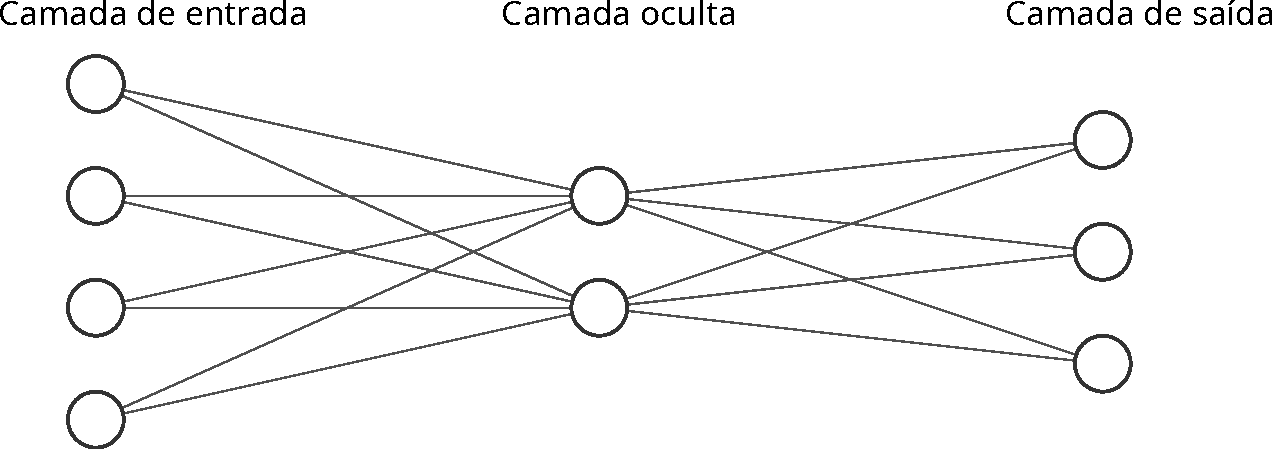
\includegraphics[scale=0.5]{Imagens/exemplo_nn}
	\end{center}
	\legend {Fonte: Autor}
\end{figure}

O neurônio é uma parte fundamental de uma ANN, nele que o aprendizado é armazenado através do reforço de conexões com
outros neurônios. Esse reforço é o peso da conexão, ele é multiplicado pela entrada e somado com os outros valores,
como é demonstrado na equação \ref{eq_neuronio} (onde $x$ é um vetor com os valores de entrada do neurônio e $w$
é um vetor com os pesos de cada entrada). Depois disso os valores passam por uma função de ativação $g(x)$ (\ref
{eq_ativacao}), que é responsável por transformar estes dados antes que sejam passados para a próxima etapa, por esta
razão, a função de ativação também é chamada função de transferência.

\begin{equation}\label{eq_neuronio}
u = \sum x_i w_i
\end{equation}
\begin{equation}\label{eq_ativacao}
y = g(u + b)
\end{equation}

\begin{figure}[htb]
	\caption {\label{cap_conceitos_ex_neuronio} Exemplo de um neurônio artificial}
	\begin{center}
		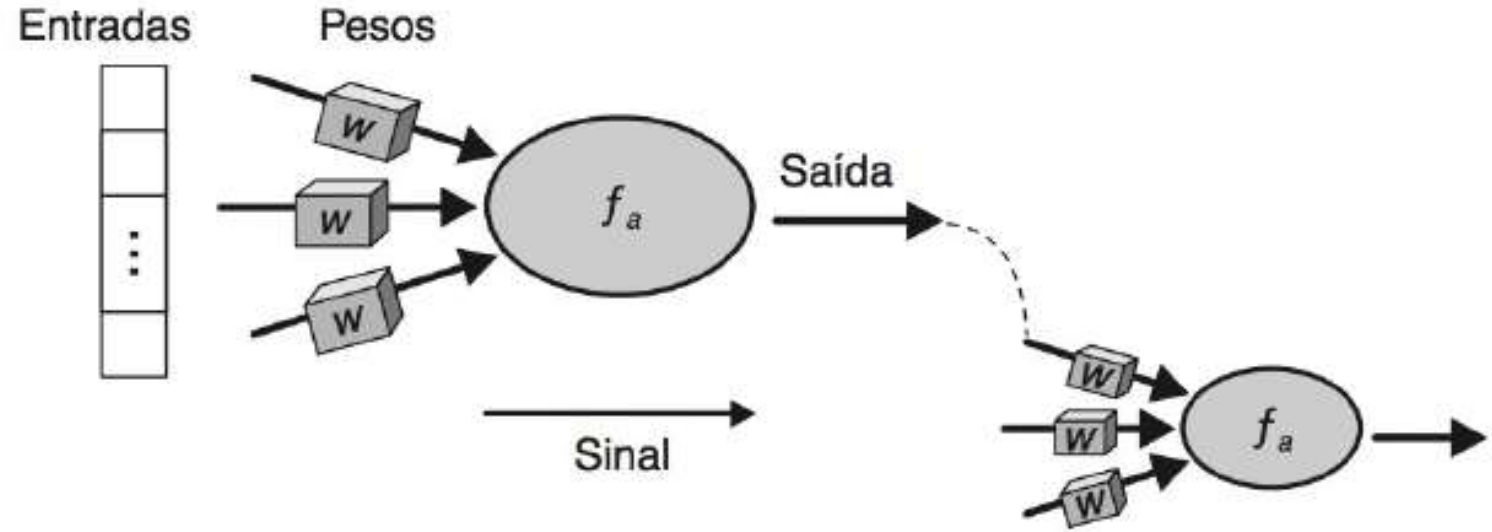
\includegraphics[scale=0.3]{Imagens/exemplo_neuronio_artificial}
	\end{center}
	\legend{Fonte: \cite{ml-faceli}}
\end{figure}

\section{Redes Neurais Convolucionais}\label{cap_conceitos_cnn}
% ---
Redes Neurais Convolucionais são Redes Neurais Artificiais que utilizam a operação de convolução para o processamento e
análise de dados no formato de \textit{grid} (grade).
Por exemplo, uma série temporal que pode ser representada no formato de \textit{grid} 1-D, ou uma imagem, que pode ser
representada no formato 2-D. \cite{Goodfellow-et-al-2016}

A arquitetura de uma CNN é composta por camadas convolucionais (\ref{cap_conceitos_cnn_conv}),
\textit{pooling} (\ref{cap_conceitos_cnn_pooling}) e totalmente conectadas (\ref{cap_conceitos_cnn_totalmente}),
como pode ser visto na \autoref{exemplo_lenet}.

\begin{figure}[htb]
	\caption {\label{exemplo_lenet} Arquitetura da LeNet}
	\begin{center}
		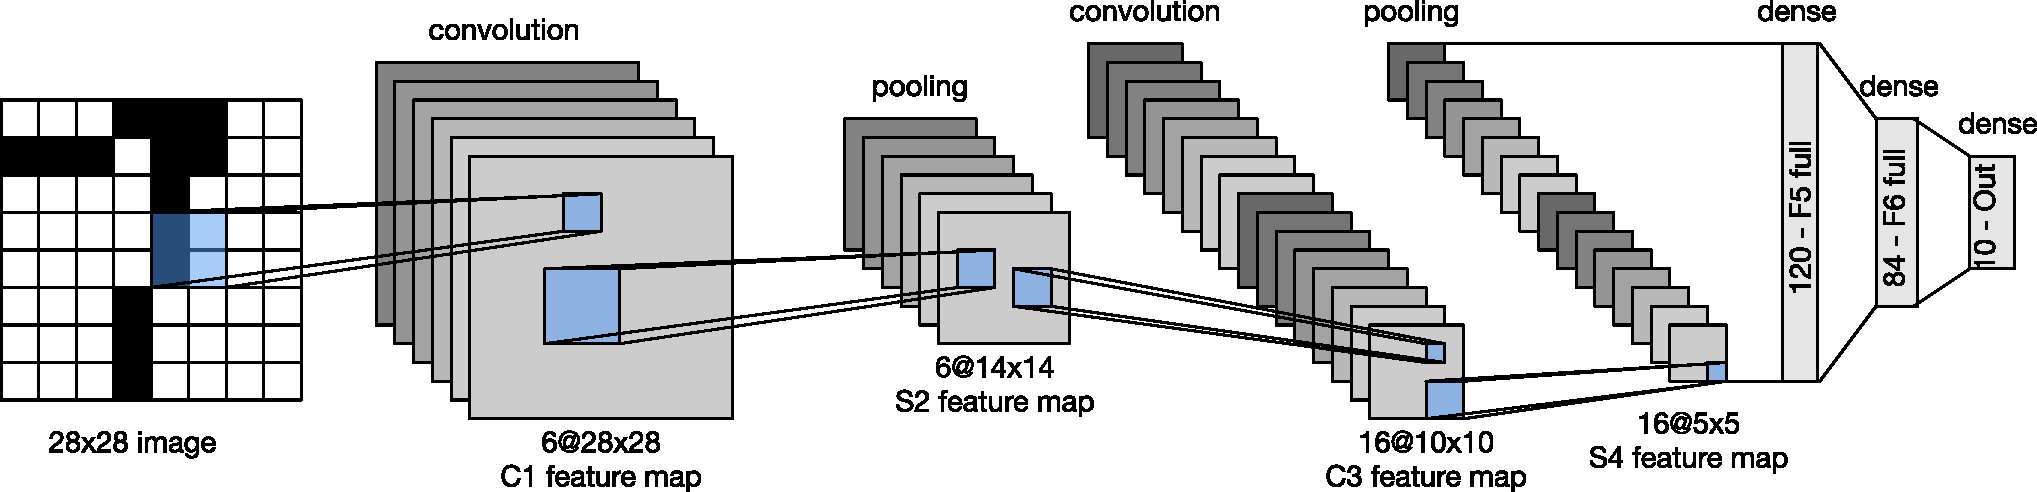
\includegraphics[scale=0.5]{Imagens/lenet}
	\end{center}
	\legend{Fonte: \cite{zhang2023dive}}
\end{figure}

\subsection{Camada de Convolução}\label{cap_conceitos_cnn_conv}
Nessa camada são aplicados filtros (matriz de pesos) nos dados de entrada, onde esses filtros deslizam ao longo da grade de
entrada executando operações de multiplicação e soma em cada elemento da matriz de entrada, com o objetivo de gerar um mapa de
características (\textit{feature map}).
O objetivo desses filtros é realçar as características dos dados de entrada. Alguns padrões como curvas e linhas podem ser
reconhecidos por estas operações de filtragem.
A \autoref{exemplo_conv}, é um exemplo da operação de convolução sendo aplicada em uma matriz.
% TODO: Adicionar figuras, referências e detalhar mais

\begin{figure}[htb]
	\caption {\label{exemplo_conv} Exemplo de convolução}
	\begin{center}
		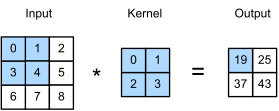
\includegraphics[scale=1.0]{Imagens/conv}
	\end{center}
	\legend{Fonte: \cite{zhang2023dive}}
\end{figure}

\subsection{Camada de \textit{pooling}}\label{cap_conceitos_cnn_pooling}
% ---
A abordagem da camada de \textit{pooling} é um pouco parecida com a camada de convolução,
uma matriz desliza pelas células da imagem, salvando apenas um dos valores dessa área na matriz de saída.
Esta operação reduz o tamanho da matriz de entrada, fazendo com que o poder computacional necessário seja reduzido,
junto com o uso de memória.

Existem diversos tipos de \textit{pooling}, min, \textit{average} e max, onde cada um foca em extrair um valor dos
dados de entrada na matriz. O tipo mais comum de \textit{pooling} é o max, que salva apenas o maior valor da área,
além de reduzir o tamanho da matriz de entrada ele consegue realçar algumas características mais expressivas da matriz.
A \autoref{exemplo_pooling} demonstra uma operação de max \textit{pooling} em uma matriz.

\begin{figure}[htb]
	\caption {\label{exemplo_pooling} Exemplo de max \textit{pooling}}
	\begin{center}
		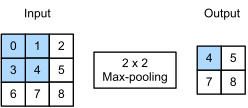
\includegraphics[scale=1.0]{Imagens/maxpooling}
	\end{center}
	\legend{Fonte: \cite{zhang2023dive}}
\end{figure}

\subsection{Camada totalmente conectada}\label{cap_conceitos_cnn_totalmente}
% ---
A camada totalmente conectada (\textit{fully connected layer}) é a camada final de uma CNN.
Depois das camadas anteriores extraírem as características da imagem, ela é responsável por
fazer aprender a interpretar essas características e inferir um resultado a partir do seu treinamento.
Onde essa camada é uma ANN (\autoref{cap_conceitos_ann}) que geralmente é focada em realizar a classificação dos dados
de entrada.

\section{\textit{Data augmentation}}\label{cap_conceitos_data_augmentation}
% ---
CNNs tem um ótimo desempenho em tarefas de visão computacional. Entretanto esse tipo de rede neural precisa de uma
grande quantidade dados para não sofrer de \textit{overfitting} (superajuste). \cite{shorten2019survey}
Esse é o objetivo do \textit{data augmentation} (aumento de dados), gerar mais dados a partir de um conjunto de dados
que já existe, aplicando algumas transformações geométricas ou espaciais, ou realizando injeção de ruído nas imagens
originais.

Na \autoref{cap_conceitos_exemplo_da}, temos um exemplo de uma imagem que sofreu uma transformação para efetuar um \textit{data augmentation}.
Nesse caso, temos uma que foi revertida (\textit{flip}), gerando um novo dado para o \text{dataset}

\begin{figure}[htb]
	\caption {\label{cap_conceitos_exemplo_da}Exemplo de uma transformação utilizando \textit{data augmentation}}
	\begin{center}
		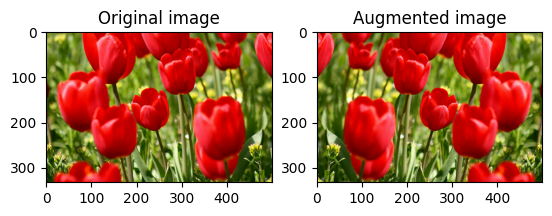
\includegraphics[scale=1]{Imagens/exemplo_da}
	\end{center}
	\legend {Fonte: \cite{tf2guia}}
\end{figure}

\section{Transferência de conhecimento}\label{cap_conceitos_transferencia}
% ---
Transferência de conhecimento consiste em usar um modelo pré-treinado em uma base de dados específica e aproveitar
o conhecimento adquirido durante esse treinamento para um novo conjunto de dados.
É necessário que o problema do \textit{dataset} (conjunto de dados) atual seja um subconjunto do \textit{dataset}
que foi usado para treinar o modelo base.

Para realizar a transferência de conhecimento é necessário adaptar a camada de entrada e de saída
(totalmente conectada) do modelo base, para que ocorra um pré-processamento dos dados de entrada
(antes deles serem passados para o modelo base), além disso é necessário definir e treinar a camada totalmente
conectada com o \textit{dataset} do problema.

\section{Métodos de compressão para Redes Neurais}\label{cap_conceitos_compressao_redes}
ANNs são utilizadas em várias aplicações, demonstrando habilidades extraordinárias no campo de visão computacional.
No entanto, redes com arquiteturas complexas são um desafio para a implantação em tempo real e necessitam de uma
grande quantidade de energia e poder computacional \cite{LIANG2021370}.
Por causa disso foram desenvolvidos métodos para reduzir o tamanho dessas redes, as tornando mais eficiente.
Nesse trabalho os métodos de poda (\ref{poda}), quantização (\ref{quantizacao}) e destilação do conhecimento
(\ref{conceitos_destilacao}) serão usados.

\subsection{\textit{Pruning}(Poda)}\label{poda}

A poda de redes neurais tem como foco eliminar conexões ou neurônios que não apresentam uma grade contribuição para a
rede.
Essa operação, é muito vantajosa para diminuir a pegada de memória \textit{memory footprint} da rede, pois ela reduz
a quantidade de parâmetros redundantes ou que não contribuem muito para a precisão dos resultados.


A operação de poda procura pesos com valores abaixo de um determinado limiar e os muda para a zero, assim deixando
a rede neural mais esparsa, o que facilita o processo de compressão.
O processo de poda pode reduzir o superajuste da rede, uma vez que remove pesos pouco importantes ou redundantes
da rede.
Podemos dividir esse processo em dois, poda estática (\textit{static pruning}), que é realiza todas as etapas de poda
o modelo sem executar o processo de inferência, e poda dinâmica (\textit{dynamic pruning}), que é realizada junto com
o processo de execução do modelo, permitindo que os nós relevantes sejam identificados.

\begin{figure}[htb]
	\caption {\label{cap_conceitos_tipos_poda}Fluxo dos tipos de poda}
	\begin{center}
		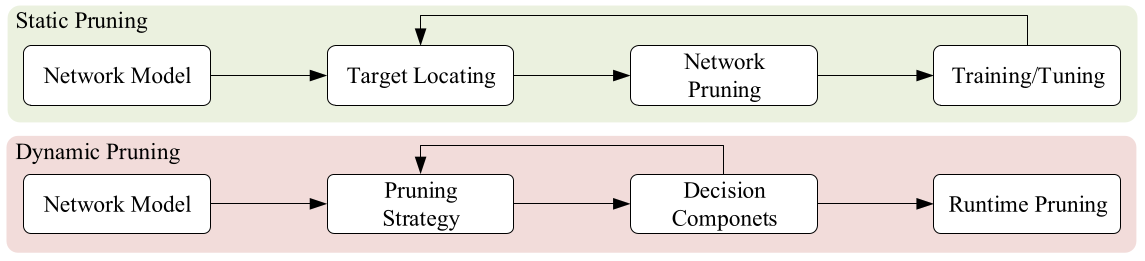
\includegraphics[scale=0.5]{Imagens/categorias-poda}
	\end{center}
	\legend {Fonte: \cite{LIANG2021370}}
\end{figure}

\subsection{Quantização}\label{quantizacao}

Quantização reduz a computação diminuindo a precisão dos tipos de dados. Pesos, \textit{bias} (vieses) e ativações
geralmente devem ser quantizadas para inteiros de 8 bit, embora implementações menores que 8 bit sejam discutidas
incluindo redes neurais binárias. \cite{LIANG2021370}

\subsection{Destilação de conhecimento (Professor-Aluno)}\label{conceitos_destilacao}

Destilação de conhecimento ou \textit{knowledge distillation} \cite{hinton2015distilling}, é uma técnica que tem
como objetivo treinar um modelo Aluno (menor e sem pré-treinamento) com um modelo Professor
(maior e com pré-treinamento). Ela é amplamente utilizada para as áreas de visão computacional e linguagem natural,
e tem como objetivo reduzir o tamanho do modelo final (Aluno).

Para transferir o conhecimento do modelo Professor para o Aluno, a técnica utiliza os \textit{logits} (entrada da
função de ativação final \textit{softmax}) no lugar da classe prevista. Além disso, são utilizado os
\textit{soft targets} (probabilidades das classes previstas pelo modelo Professor) junto com os
\textit{hard targets} (classe esperada).

% NOTE: Talvez detalhar a temperatura?

\section{Otimização Bayesiana}\label{cap_conceitos_bayesiana}
% ---
Testar diferentes valores para os hiperparâmetros é uma tarefa essencial para otimizar o desempenho de ANNs.
A otimização Bayesiana é um dos métodos utilizados para fazer esse teste, ela possui dois componentes principais,
o modelo estatístico Bayesiano, que modelar a função objetiva, e a função de aquisição, que decide a próxima amostra
de parâmetros. \cite{frazier2018tutorial}

A otimização Bayesiana procura encontrar um valor ótimo (maximizando ou minimizando alguma métrica do modelo).
Inicialmente os hiperparâmetros são escolhidos aleatoriamente e testados, após algumas iterações o modelo começa
a convergir para um resultado ótimo, em algum ponto essa função de otimização só irá escolher o melhor conjunto de
parâmetros testado.

% TODO: Refinar, sendo mais objetivo
